\addcontentsline{toc}{section}{Introduction}

\section*{Introduction}

\section{Definition}
Trino is an open source distributed SQL query engine. It is a hard fork of the original Presto project created by Facebook. It lets developers run interactive analytics against large volumes of data. With Trino, organizations can easily use their existing SQL skills to query data without having to learn new complex languages. The architecture is quite similar to traditional online analytical processing (OLAP) systems using distributed computing architectures, in which one controller node coordinates multiple worker nodes.

\section{How it works}
Trino is a distributed system that runs on Hadoop, and uses an architecture similar to massively parallel processing (MPP) databases. It has one coordinator node working with multiple worker nodes. Users submit SQL to the coordinator which uses query and execution engine to parse, plan, and schedule a distributed query plan across the worker nodes. It supports standard ANSI SQL, including complex queries, joins aggregations, and outer joins.

Leveraging this architecture, the Trino query engine is able to process SQL queries on large amounts of data in parallel across a cluster of computers, or nodes. Trino runs as a single-server process on each node. Multiple nodes running Trino, which are configured to collaborate with each other, make up a Trino cluster.

The following figure displays a high-level overview of a Trino cluster composed of one coordinator and multiple worker nodes. A Trino user connects to the coordinator with a client, such as a tool using the JDBC driver or the Trino CLI. The coordinator then collaborates with the workers, which access the data sources.

\begin{figure}[htbp]
\centering
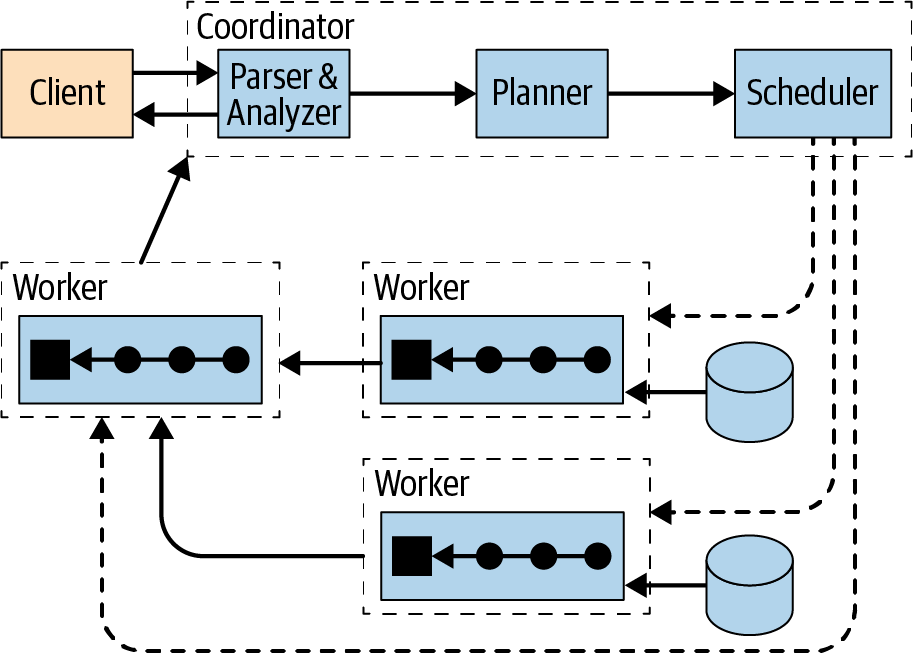
\includegraphics[width=\linewidth]{images/trino_architecture.png}
\caption{Trino architecture overview with coordinator and workers}\label{fig:trino-architecture}
\end{figure}

\begin{enumerate}
	\item A coordinator is a Trino server that handles incoming queries and manages the workers to execute the queries.
	\item A worker is a Trino server responsible for executing tasks and processing data.
	\item The discovery service typically runs on the coordinator and allows workers to register to participate in the cluster.
	\item All communication and data transfer between clients, coordinator, and workers uses REST-based interactions over HTTP/HTTPS.
\end{enumerate}

The following figure shows how the communication within the cluster happens between the coordinator and the workers, as well as from one worker to another. The coordinator talks to workers to assign work, update status, and fetch the top-level result set to return to the users. The workers talk to each other to fetch data from upstream tasks, running on other workers. And the workers retrieve result sets from the data source.


\begin{figure}[htbp]
\centering
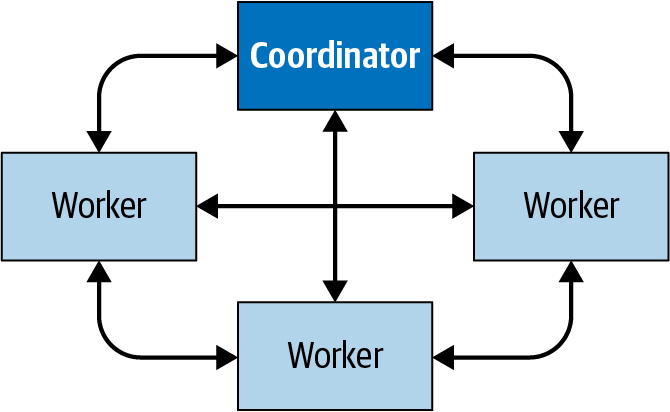
\includegraphics[width=\linewidth]{images/trino_communication.png}
\caption{Communication between coordinator and workers in a Trino cluster}\label{fig:trino-communication}
\end{figure}

\section{Coordinator}
The Trino coordinator is the server responsible for receiving SQL statements from the users, parsing these statements, planning queries, and managing worker nodes. It’s the brain of a Trino installation and the node to which a client connects. Users interact with the coordinator via the Trino CLI, applications using the JDBC or ODBC drivers, or any other available client libraries for a variety of languages. The coordinator accepts SQL statements from the client such as SELECT queries for execution.

Every Trino installation must have a coordinator alongside one or more workers. For development or testing purposes, a single instance of Trino can be configured to perform both roles.

The coordinator keeps track of the activity on each worker and coordinates the execution of a query. The coordinator creates a logical model of a query involving a series of stages.

Once it receives a SQL statement, the coordinator is responsible for parsing, analyzing, planning, and scheduling the query execution across the Trino worker nodes. The statement is translated into a series of connected tasks running on a cluster of workers. As the workers process the data, the results are retrieved by the coordinator and exposed to the clients on an output buffer. Once an output buffer is completely read by the client, the coordinator requests more data from the workers on behalf of the client. The workers, in turn, interact with the data sources to get the data from them. As a result, data is continuously requested by the client and supplied by the workers from the data source until the query execution is completed.

Coordinators communicate with workers and clients by using an HTTP-based protocol.

\begin{figure}[htbp]
\centering
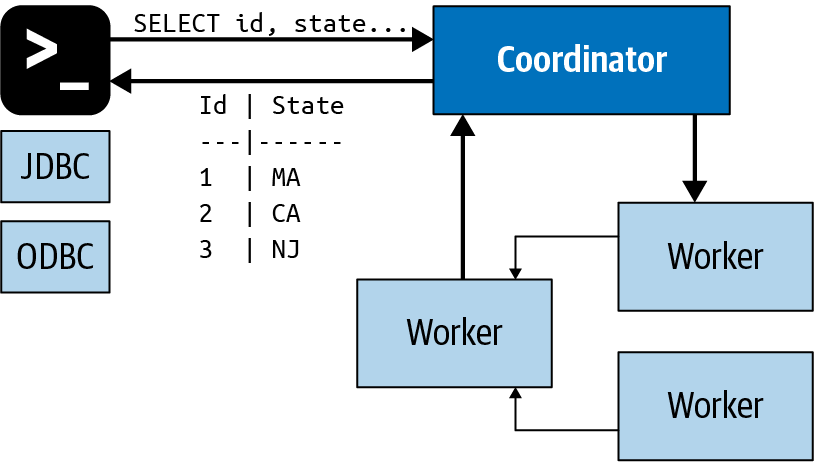
\includegraphics[width=\linewidth]{images/trino_communication_processing.png}
\caption{Client, coordinator, and worker communication processing a SQL statement}\label{fig:trino-communication-precessing}
\end{figure}

\section{Workers}
A Trino worker is a server in a Trino installation. It is responsible for executing tasks assigned by the coordinator and for processing data. Worker nodes fetch data from data sources by using connectors and then exchange intermediate data with each other. The final resulting data is passed on to the coordinator. The coordinator is responsible for gathering the results from the workers and providing the final results to the client.

During installation, workers are configured to know the hostname or IP address of the discovery service for the cluster. When a worker starts up, it advertises itself to the discovery service, which makes it available to the coordinator for task execution.

Workers communicate with other workers and the coordinator by using an HTTP-based protocol.

The following figure shows how multiple workers retrieve data from the data sources and collaborate to process the data, until one worker can provide the data to the coordinator.

\begin{figure}[htbp]
\centering
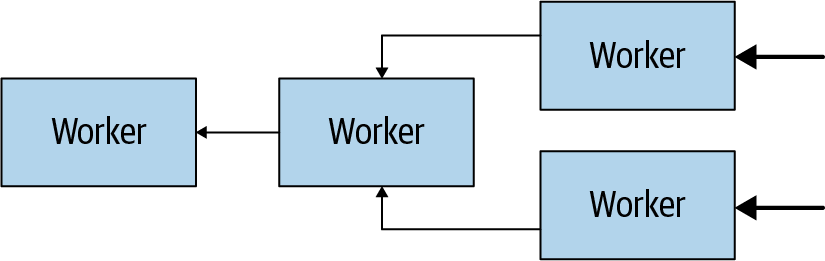
\includegraphics[width=\linewidth]{images/trino_workers.png}
\caption{Workers in a cluster collaborate to process SQL statements and data}\label{fig:trino-workers}
\end{figure}

\section{Connector-Based Architecture}
At the heart of the separation of storage and compute in Trino is the connector-based architecture. A connector provides Trino an interface to access an arbitrary data source.

Each connector provides a table-based abstraction over the underlying data source. As long as data can be expressed in terms of tables, columns, and rows by using the data types available to Trino, a connector can be created and the query engine can use the data for query processing.

Trino provides a service provider interface (SPI), which is a type of API used to implement a connector. By implementing the SPI in a connector, Trino can use standard operations internally to connect to any data source and perform operations on any data source. The connector takes care of the details relevant to the specific data source.

At the heart of the separation of storage and compute in Trino is the connector-based architecture. A connector provides Trino an interface to access an arbitrary data source.

Each connector provides a table-based abstraction over the underlying data source. As long as data can be expressed in terms of tables, columns, and rows by using the data types available to Trino, a connector can be created and the query engine can use the data for query processing.

Trino provides a service provider interface (SPI), which is a type of API used to implement a connector. By implementing the SPI in a connector, Trino can use standard operations internally to connect to any data source and perform operations on any data source. The connector takes care of the details relevant to the specific data source.
\begin{enumerate}
	\item[$\bullet$] Operations to fetch table/view/schema metadata
	\item[$\bullet$] Operations to produce logical units of data partitioning, so that Trino can parallelize reads and writes
	\item[$\bullet$] Data sources and sinks that convert the source data to/from the in-memory format expected by the query engine 
\end{enumerate}

Trino provides many connectors to systems, here are the list of connects as of the writing of this report:

% chktex-file 44
\begin{table}[ht]
\centering
	\begin{tabular}{|c|c|}
	\hline
	\textbf{Connector Name} & \textbf{Documentation Link} \\ \hline
	Accumulo & \href{https://trino.io/docs/current/connector/accumulo.html}{https://trino.io/docs/current/connector/accumulo.html} \\ \hline
	Atop & \href{https://trino.io/docs/current/connector/atop.html}{https://trino.io/docs/current/connector/atop.html} \\ \hline
	BigQuery & \href{https://trino.io/docs/current/connector/bigquery.html}{https://trino.io/docs/current/connector/bigquery.html} \\ \hline
	Black Hole & \href{https://trino.io/docs/current/connector/blackhole.html}{https://trino.io/docs/current/connector/blackhole.html} \\ \hline
	Cassandra & \href{https://trino.io/docs/current/connector/cassandra.html}{https://trino.io/docs/current/connector/cassandra.html} \\ \hline
	ClickHouse & \href{https://trino.io/docs/current/connector/clickhouse.html}{https://trino.io/docs/current/connector/clickhouse.html} \\ \hline
	Delta Lake & \href{https://trino.io/docs/current/connector/delta-lake.html}{https://trino.io/docs/current/connector/delta-lake.html} \\ \hline
	Druid & \href{https://trino.io/docs/current/connector/druid.html}{https://trino.io/docs/current/connector/druid.html} \\ \hline
	Elasticsearch & \href{https://trino.io/docs/current/connector/elasticsearch.html}{https://trino.io/docs/current/connector/elasticsearch.html} \\ \hline
	Google Sheets & \href{https://trino.io/docs/current/connector/googlesheets.html}{https://trino.io/docs/current/connector/googlesheets.html} \\ \hline
	Hive & \href{https://trino.io/docs/current/connector/hive.html}{https://trino.io/docs/current/connector/hive.html} \\ \hline
	Hudi & \href{https://trino.io/docs/current/connector/hudi.html}{https://trino.io/docs/current/connector/hudi.html} \\ \hline
	Iceberg & \href{https://trino.io/docs/current/connector/iceberg.html}{https://trino.io/docs/current/connector/iceberg.html} \\ \hline
	Ignite & \href{https://trino.io/docs/current/connector/ignite.html}{https://trino.io/docs/current/connector/ignite.html} \\ \hline
	JMX & \href{https://trino.io/docs/current/connector/jmx.html}{https://trino.io/docs/current/connector/jmx.html} \\ \hline
	Kafka & \href{https://trino.io/docs/current/connector/kafka.html}{https://trino.io/docs/current/connector/kafka.html} \\ \hline
	Kinesis & \href{https://trino.io/docs/current/connector/kinesis.html}{https://trino.io/docs/current/connector/kinesis.html} \\ \hline
	Kudu & \href{https://trino.io/docs/current/connector/kudu.html}{https://trino.io/docs/current/connector/kudu.html} \\ \hline
	Local File & \href{https://trino.io/docs/current/connector/localfile.html}{https://trino.io/docs/current/connector/localfile.html} \\ \hline
	MariaDB & \href{https://trino.io/docs/current/connector/mariadb.html}{https://trino.io/docs/current/connector/mariadb.html} \\ \hline
	Memory & \href{https://trino.io/docs/current/connector/memory.html}{https://trino.io/docs/current/connector/memory.html} \\ \hline
	MongoDB & \href{https://trino.io/docs/current/connector/mongodb.html}{https://trino.io/docs/current/connector/mongodb.html} \\ \hline
	MySQL & \href{https://trino.io/docs/current/connector/mysql.html}{https://trino.io/docs/current/connector/mysql.html} \\ \hline
	Oracle & \href{https://trino.io/docs/current/connector/oracle.html}{https://trino.io/docs/current/connector/oracle.html} \\ \hline
	Phoenix & \href{https://trino.io/docs/current/connector/phoenix.html}{https://trino.io/docs/current/connector/phoenix.html} \\ \hline
	Pinot & \href{https://trino.io/docs/current/connector/pinot.html}{https://trino.io/docs/current/connector/pinot.html} \\ \hline
	PostgreSQL & \href{https://trino.io/docs/current/connector/postgresql.html}{https://trino.io/docs/current/connector/postgresql.html} \\ \hline
	Prometheus & \href{https://trino.io/docs/current/connector/prometheus.html}{https://trino.io/docs/current/connector/prometheus.html} \\ \hline
	Redis & \href{https://trino.io/docs/current/connector/redis.html}{https://trino.io/docs/current/connector/redis.html} \\ \hline
	Redshift & \href{https://trino.io/docs/current/connector/redshift.html}{https://trino.io/docs/current/connector/redshift.html} \\ \hline
	SingleStore & \href{https://trino.io/docs/current/connector/singlestore.html}{https://trino.io/docs/current/connector/singlestore.html} \\ \hline
	SQL Server & \href{https://trino.io/docs/current/connector/sqlserver.html}{https://trino.io/docs/current/connector/sqlserver.html} \\ \hline
	System & \href{https://trino.io/docs/current/connector/system.html}{https://trino.io/docs/current/connector/system.html} \\ \hline
	Thrift & \href{https://trino.io/docs/current/connector/thrift.html}{https://trino.io/docs/current/connector/thrift.html} \\ \hline
	TPCDS & \href{https://trino.io/docs/current/connector/tpcds.html}{https://trino.io/docs/current/connector/tpcds.html} \\ \hline
	TPCH & \href{https://trino.io/docs/current/connector/tpch.html}{https://trino.io/docs/current/connector/tpch.html} \\ \hline
\end{tabular}
\caption{List of Trino Connectors and their documentation}
\end{table}

Trino’s SPI also gives you the ability to create your own custom connectors. This may be needed if you need to access a data source without a compatible connector. If you end up creating a connector, we strongly encourage you to learn more about the Trino open source community, use our help, and contribute your connector. Check out “Trino Resources” for more information. A custom connector may also be needed if you have a unique or proprietary data source within your organization. This is what allows Trino users to query any data source by using SQL—truly SQL-on-Anything.

The following figure shows how the Trino SPI includes separate interfaces for metadata, data statistics, and data location used by the coordinator, and for data streaming used by the workers

\begin{figure}[htbp]
\centering
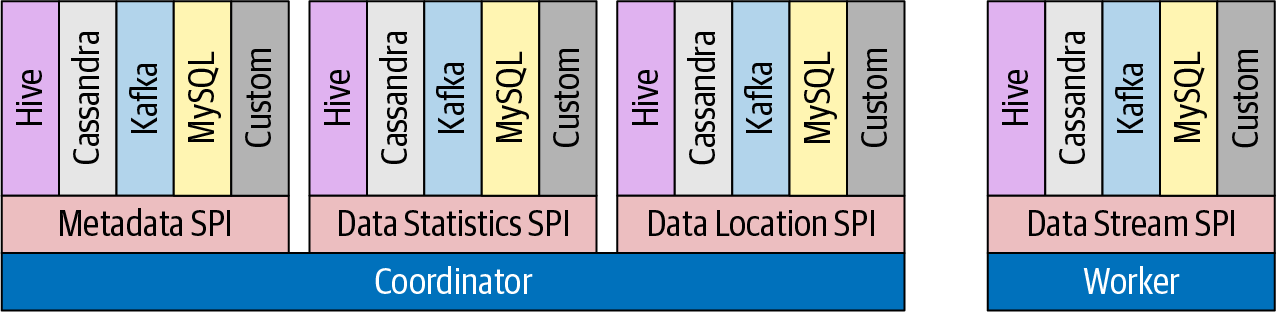
\includegraphics[width=\linewidth]{images/trino_connector.png}
\caption{Overview of the Trino service provider interface (SPI)}\label{fig:trino-connector}
\end{figure}

Trino connectors are plug-ins loaded by each server at startup. They are configured by specific parameters in the catalog properties files and loaded from the plug-ins directory. 

\section{Catalogs, Schemas, and Tables}
The Trino cluster processes all queries by using the connector-based architecture described earlier. Each catalog configuration uses a connector to access a specific data source. The data source exposes one or more schemas in the catalog. Each schema contains tables that provide the data in table rows with columns using different data types. You can find out more about catalogs, schemas, tables. Specifically in “Catalogs”, “Schemas”, and “Tables”.


\addcontentsline{toc}{section}{Conclusion}
\section*{Conclusion}
The Trino architecture has a coordinator receiving user requests and then using workers to assemble all the data from the data sources. Each query is translated into a distributed query plan of tasks in numerous stages. The data is returned by the connectors in splits and processed in multiple stages until the final result is available and provided to the user by the coordinator.